%% ****** Start of file apstemplate.tex ****** %
%%
%%
%%   This file is part of the APS files in the REVTeX 4 distribution.
%%   Version 4.1r of REVTeX, August 2010
%%
%%
%%   Copyright (c) 2001, 2009, 2010 The American Physical Society.
%%
%%   See the REVTeX 4 README file for restrictions and more information.
%%
%
% This is a template for producing manuscripts for use with REVTEX 4.0
% Copy this file to another name and then work on that file.
% That way, you always have this original template file to use.
%
% Group addresses by affiliation; use superscriptaddress for long
% author lists, or if there are many overlapping affiliations.
% For Phys. Rev. appearance, change preprint to twocolumn.
% Choose pra, prb, prc, prd, pre, prl, prstab, prstper, or rmp for journal
%  Add 'draft' option to mark overfull boxes with black boxes
%  Add 'showpacs' option to make PACS codes appear
%  Add 'showkeys' option to make keywords appear
\documentclass[aps,prl,twocolumn,groupedaddress]{revtex4-1}
%\documentclass[aps,prl,preprint,superscriptaddress]{revtex4-1}
%\documentclass[aps,prl,reprint,groupedaddress]{revtex4-1}

% You should use BibTeX and apsrev.bst for references
% Choosing a journal automatically selects the correct APS
% BibTeX style file (bst file), so only uncomment the line
% below if necessary.

\usepackage{graphicx}
\usepackage[caption=false]{subfig}
\usepackage{braket}
\usepackage{mathtools}
\graphicspath{{figures/}}
\DeclareMathOperator{\sinc}{sinc}

\begin{document}

% Use the \preprint command to place your local institutional report
% number in the upper righthand corner of the title page in preprint mode.
% Multiple \preprint commands are allowed.
% Use the 'preprintnumbers' class option to override journal defaults
% to display numbers if necessary
%\preprint{}

%Title of paper
\title{Force and Amplitude Sensing with Ions in a Penning Trap}

% repeat the \author .. \affiliation  etc. as needed
% \email, \thanks, \homepage, \altaffiliation all apply to the current
% author. Explanatory text should go in the []'s, actual e-mail
% address or url should go in the {}'s for \email and \homepage.
% Please use the appropriate macro foreach each type of information

% \affiliation command applies to all authors since the last
% \affiliation command. The \affiliation command should follow the
% other information
% \affiliation can be followed by \email, \homepage, \thanks as well.
\author{K. A. Gilmore}
\email[]{kevin.gilmore@colorado.edu}
%\homepage[]{Your web page}
%\thanks{}
%\altaffiliation{}
\affiliation{National Institute of Standards and Technology, JILA, and Department of Physics, University of Colorado, Boulder, Colorado, 80309, USA}

\author{J. G. Bohnet}
\author{J. J. Bollinger}
\affiliation{National Institute of Standards and Technology, Boulder, Colorado 80305, USA}

%Collaboration name if desired (requires use of superscriptaddress
%option in \documentclass). \noaffiliation is required (may also be
%used with the \author command).
%\collaboration can be followed by \email, \homepage, \thanks as well.
%\collaboration{}
%\noaffiliation

\date{\today}

\begin{abstract}
\end{abstract}

% insert suggested PACS numbers in braces on next line
\pacs{}
% insert suggested keywords - APS authors don't need to do this
%\keywords{}

%\maketitle must follow title, authors, abstract, \pacs, and \keywords
\maketitle

% If in two-column mode, this environment will change to single-column
% format so that long equations can be displayed. Use
% sparingly.
%\begin{widetext}
% put long equation here
%\end{widetext}

% figures should be put into the text as floats.
% Use the graphics or graphicx packages (distributed with LaTeX2e)
% and the \includegraphics macro defined in those packages.
% See the LaTeX Graphics Companion by Michel Goosens, Sebastian Rahtz,
% and Frank Mittelbach for instance.
%
% Here is an example of the general form of a figure:
% Fill in the caption in the braces of the \caption{} command. Put the label
% that you will use with \ref{} command in the braces of the \label{} command.
% Use the figure* environment if the figure should span across the
% entire page. There is no need to do explicit centering.

% \begin{figure}
% \includegraphics{}%
% \caption{\label{}}
% \end{figure}

% Surround figure environment with turnpage environment for landscape
% figure
% \begin{turnpage}
% \begin{figure}
% \includegraphics{}%
% \caption{\label{}}
% \end{figure}
% \end{turnpage}

% tables should appear as floats within the text
%
% Here is an example of the general form of a table:
% Fill in the caption in the braces of the \caption{} command. Put the label
% that you will use with \ref{} command in the braces of the \label{} command.
% Insert the column specifiers (l, r, c, d, etc.) in the empty braces of the
% \begin{tabular}{} command.
% The ruledtabular enviroment adds doubled rules to table and sets a
% reasonable default table settings.
% Use the table* environment to get a full-width table in two-column
% Add \usepackage{longtable} and the longtable (or longtable*}
% environment for nicely formatted long tables. Or use the the [H]
% placement option to break a long table (with less control than 
% in longtable).
% \begin{table}%[H] add [H] placement to break table across pages
% \caption{\label{}}
% \begin{ruledtabular}
% \begin{tabular}{}
% Lines of table here ending with \\
% \end{tabular}
% \end{ruledtabular}
% \end{table}

% Surround table environment with turnpage environment for landscape
% table
% \begin{turnpage}
% \begin{table}
% \caption{\label{}}
% \begin{ruledtabular}
% \begin{tabular}{}
% \end{tabular}
% \end{ruledtabular}
% \end{table}
% \end{turnpage}


% body of paper here - Use proper section commands
% References should be done using the \cite, \ref, and \label commands
\section{Introduction}
% Put \label in argument of \section for cross-referencing
%\section{\label{}}
Well controlled and understood quantum systems offer advantages over their classical counterparts and are finding uses in a variety of up-and-coming disciplines. Quantum information and quantum cryptography are chief among them, but the use of such a quantum mechanical system as a sensor may prove to be as useful as the advent of semiconductors on sensing technology. Quantum metrology, where the sensing protocol is enhanced by entanglement, is the most direct way to improve a measurement’s sensitivity beyond the classical limit. However, such methods remain relatively far from useful application. The use of a quantum system sensitive to a physical parameter, such as an electric or magnetic field, is of more immediate usefulness for sensitive measurements. Cavity-based optomechanical resonators have proven to be tremendously sensitive to a wide variety of physical parameters and are the most prominent example of a meso/macro-scopic system used as a quantum sensor. Single ion sensors make use of their long coherence times to make measurements and are the prime example of a single quantum object used as a sensor. Our 2-D crystal of ions in a Penning trap operates in a regime between these two paradigms. By scaling up the number of ions we see an increase in sensitivity to ion displacement and electric fields compared to a single ion. Though our experiments are performed phase-incoherently and off-resonantly, with near-term improvements we expect to operate phase-coherently and on resonance with the center of mass mode frequency of the ion crystal. This would enable us to make use of recently demonstrated spin-squeezing in our ensemble of 100s of ions to perform further quantum enhanced sensing. As it stands, we are able to detect a displacement of 200 pm due to an RF drive applied to the trap endcap electrode. The ground state wavefunction size is 10 nm, 50 times as large.

What these different experimental setups have in common as sensors is that they all make use of a mechanical oscillator. An ion in an RF trap oscillates at the trap resonance frequency. A microfabricated resonator is an oscillating membrane. The ion crystal in an Penning trap behaves like both: the drumhead modes of the crystal oscillate like a membrane with the center of mass mode at the trap resonance frequency. The sensing of an applied drive is done by measuring the displacement of the oscillator. Naturally, the best force sensitivity for such a mechanical oscillator occurs when the applied force is driven at the resonance frequency. Driving the oscillator with a small, off-resonant force requires greater displacement sensitivity - as the same force applied on resonance results in a much larger displacement. In addition, the standard quantum limit (SQL) and fundamental quantum limit (QL) converge at the resonance, but off-resonance the SQL may be surpassed. By operating off-resonantly, we can demonstrate in the future with phase-coherent detection amplitude sensing below the SQL.
\section{Experimental Setup}
Our experimental apparatus consists of $\prescript{9}{}{}$Be$^{+}$ ions confined to a single-plane Coulomb crystal in a Penning trap, described in Fig. 1 and (ref). The ions are cooled to the Doppler limit and the scattered fluorescence is used for imaging. The spin-1/2 system is the $\prescript{2}{}{S}_{1/2}$ ground state of the valence electron spin $\ket{\uparrow} (\ket{\downarrow}) \equiv \ket{m_{s}=+1/2} (\ket{m_{s}=-1/2}) $. In the magnetic field of the Penning trap, the ground state is split by 124 GHz. A resonant microwave source is used to perform global rotations of the spin ensemble. A pair of off-resonant laser beams generate a spin-dependent optical dipole force, coupling the spins to the ions's axial motion. The spins can be used as a sensitive readout of the axial motion.
\begin{figure}
  \subfloat[]{%
    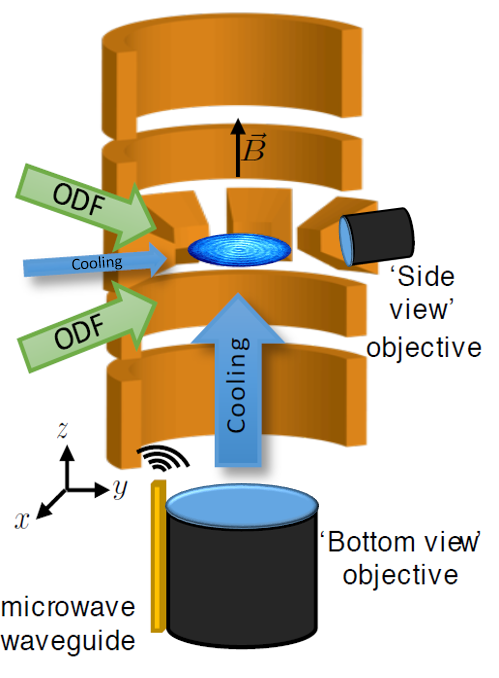
\includegraphics[width=.25\textwidth]{penning_trap}}\hfill
  \subfloat[]{%
    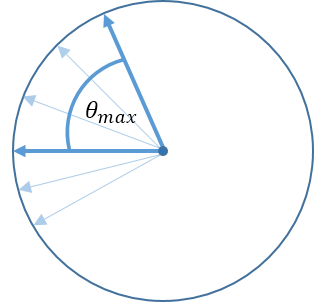
\includegraphics[width=.15\textwidth]{dumb_dephasing}}
  \caption{(a) Cross-section of the NIST Penning trap, characterized by an axial magnetic field $B = 4.45$ T and an axial trap frequency $\omega_z = 2\pi \times 1.57$ MHz. The blue disk represents the ion crystal. Cylindrical electrodes (orange) generate a harmonic confining potential along their axis. Radial confinement is provided by the Lorentz force from $\vec{E} \times \vec{B}$-induced rotation in the axial magnetic field. Time varying potentials applied to eight azimuthally segmented electrodes generate a rotating wall potential that controls the crystal rotation frequency. Doppler cooling beams are directed along $y$ and $z$. The beams responsible for the spin-dependent optical dipole force are at $10^{\circ} $ from the ion plane. Global, state-dependent fluoresence is collected on the side-view objective. (b) After rotating to the equator on the Bloch sphere, an incoherent axial perturbation causes precession. The maximum precessed angle is $\theta_{max}$. }\label{fig:1}
\end{figure}

By measuring the decrease in the composite Bloch vector length produced by the application of a homogenous spin-dependent force, detailed information about the motional state of the ions is revealed. This spin dephasing is directly measured. The spin-dependent optical dipole force (ODF) is generated from the interference of a pair of detuned lasers, shown in Fig. 1a. The ODF couples the spin and motional degrees of freedom through the interaction 
\begin{equation}
H_{ODF} = U\sum_{i}\sin(\delta k \cdot z_i - \mu t + \phi)\sigma^{z}_i,
\end{equation}
where $\delta k$ is the wave vector, $\mu/2\pi$ is the beatnote frequency, and $\phi$ is the phase between the ODF beams, and $z_i$ and $\sigma^{z}_i$ are the position operator and Pauli spin matrix for ion $i$. This Hamiltonian may be rewritten, ignoring very low frequencies $\mu$, as
\[H_{ODF} = U\sum_{i}\sin(\delta k \cdot z_i)\cos(\mu t + \phi)\sigma^{z}_i. \]
Tuning the ODF difference frequency allows for readout of the motional state of the ions at that frequency by measuring the precession of the spins about the Bloch sphere and, in a typical Ramsey style experiment, projecting this on to the dark state (spin-down). Spin-dephasing, then, appears as an increase in spin-up population. The precession due to an axial oscillation can be determined by considering a classical driven motion of constant amplitude $z_{0}$, frequency $\omega$, and phase $\delta$, $z_i \rightarrow z_i +z_0\cos(\omega t+\delta)$.
Then,
\[H_{ODF} = DWF \cdot U \cdot \delta k \cdot z_0\cos((\omega - \mu)t + \delta + \phi) \sum_{i} \frac{\sigma^{z}_{i}}{2} \]
where $DWF = \exp(-\delta k^2 \left< z^{2}_{i} \right> / 2) $.
For the case $ \omega = \mu $, where the ODF frequency difference is equal to the frequency of the applied drive,
\[\theta = \Delta\tau = DWF \cdot U \cdot \delta k \cdot z_0 \cdot \tau \cos(\delta - \phi) = \theta_{max}\cos(\delta - \phi)\]
where $\Delta$ is the energy difference between spin-up and spin-down for each ion and $\tau$ is the total ODF interaction time. $\theta_{max}$ is the maximum precession, which occurs when the drive is in phase with the ODF beatnote.

Due to current experimental limitations, we do our measurements phase incoherently. However, where the phase of the applied force unknown or time-dependent, this phase-incoherent sensing would be necessary - and so, our experiment represents a 'worse-case' sensing experiment. In the phase-incoherent picture, the different relative phases between the drive and beatnote are sampled randomly with each repetition of the experiment. Despite this, one can extract the maximum precession angle, $\theta_{max}$. In a Ramsey sequence where the Bloch vector with no precession is rotated down to the dark state, the component along $-\hat{z}$ has length $\cos(\theta)$. Thus the probability for measuring spin-up is $P_{\uparrow} = \frac{1}{2}[1-e^{-\Gamma \tau} \cos(\theta)]$, where $\tau$ is the total ODF interaction time and $\Gamma = \frac{1}{2}(\Gamma_{el} + \Gamma_{ram})$ is the spontaneous decay rate where $\Gamma_{el}$ ($\Gamma_{ram}$) is the elastic (Raman) scattering decoherence rate (Uys PRL ref). To model the phase incoherent experiment, one must average over this length, $ \left< \cos(\theta) \right> $. It can be shown that $ \left< \cos(\theta) \right> = J_0(\theta_{max}) $, where $J_0$ is the zeroth order Bessel function of the first kind. Thus,
\begin{equation}
\left< P_{\uparrow} \right> = \frac{1}{2} \left[ 1-e^{-\Gamma \tau}J_0(\theta_{max}) \right].
\end{equation}
To create an axial oscillation, we apply an AC voltage to the endcap of the Penning trap. This can be done either on-resonance or off-resonance with the center of mass mode of the ion crystal at $2\pi \times 1.57$ MHz. Characterization of the detection sensitivity requires calibration of the applied drive in terms of ion displacement. To calibrate the displacement of the ions as a result of this applied drive, we apply a static voltage to the endcap and measure the deflection of the ion crystal. The deflection is measured using an f/10 light collection system and a CCD camera, which provides spatial resolution of $\sim .8 \mu$m per pixel. From this calibration, we find 1 V results in 0.97 $\pm$ 0.009 $\mu$m of displacement.
\begin{figure*}
  \subfloat[]{%
    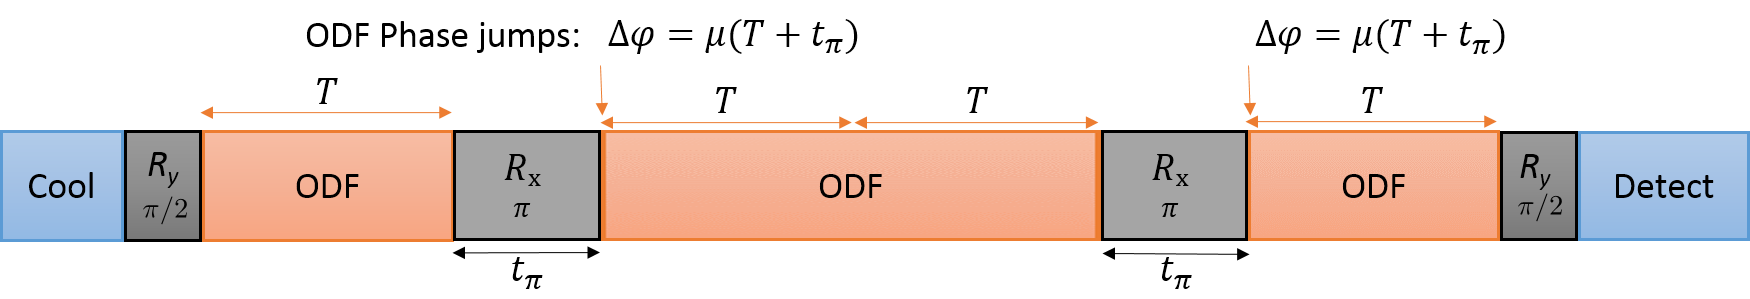
\includegraphics[width=.8\textwidth]{cpmg}}\\
  \subfloat[]{%
    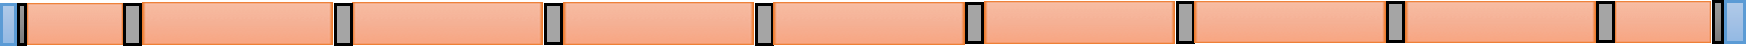
\includegraphics[width=.8\textwidth]{8pi_cpmg}}\\
  \subfloat[]{%
    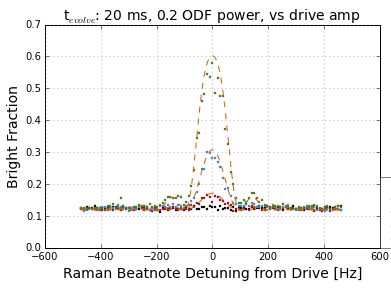
\includegraphics[width=.45\textwidth]{lineshape_vs_drive}}\hfill
  \subfloat[]{%
    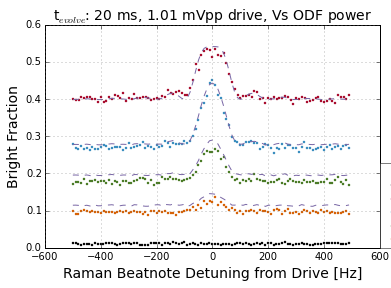
\includegraphics[width=.45\textwidth]{lineshape_vs_odf}}
  \caption{(a) CPMG sequence with 2 $\pi$ pulses. Orange blocks represent ODF pulses, grey microwave rotations, and blue cooling and detecting. In this experiment, the classical drive is left on throughout. After each $\pi$ pulse, the ODF phase is jumped in order to sum the phases accumulated in each ODF arm. (b) CPMG sequence with 8 $\pi$ pulses. Cooling and detection remain the same, and the phase is jumped by the same amount after each $\pi$ pulse. Chaining the ODF pulses in this fashion allows us to go to much longer total interaction times (20 ms) and detect much smaller induced displacements. (c) Lineshape of the classical drive for drive amplitudes of 500 pm (red), 1 nm (green) and 2 nm (purple). Black points are background, with drive turned off. Dashed lines are theory curves with no free parameters.  (d) Lineshape for classical drive displacement of 500 pm and  fractional ODF power of 1 (red), 0.5 (green), 0.3 (purple), and 0.15 (dark green). As the ODF power is increased, the background rises and the optimal signal-to-noise is found.}\label{fig:2}
\end{figure*}
\begin{figure}
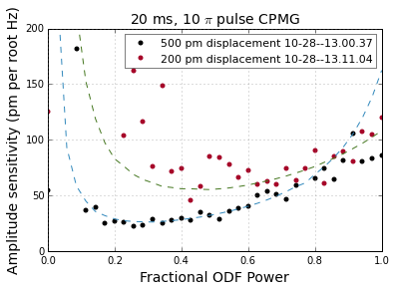
\includegraphics[width=.25\textwidth]{amp_sense_both}
\caption{Amplitude sensitivity as a function of ODF power. There is an optimal signal-to-noise that occurs before the background begins to dominate. We calculate a minimum sensitivity of $\sim$25 pm per root Hz.}\label{Fig 3}
\end{figure}
\section{Off-resonance amplitude sensing}
By applying a ~400kHz drive to the endcap electrode, we can study the response of the ion harmonic oscillator to an off resonant force. A spin echo sequence is used to decouple from magnetic field fluctuations over the course of the experimental sequence. To extend the sequence out to long time in order to detect more sensitively, a CPMG style sequence is used. Our experimental sequence makes use of the quantum lock-in technique wherein the phase accumulated in each arm of the sequence is added coherently. Figure 2 shows a CPMG sequence with 2 $\pi$ pulses and phase jumps appropriate for adding the phases. Adding in 6 additional $\pi$ pulses and ODF pulses allows us to push the sequence time out to 20 ms and maintain a background fully characterized by decoherence due to spontaneous emission.

To model the lineshape of the signal, it is necessary to account for the accumulated phase due to the spin-dependent ODF potential without making the simplification that $ \omega = \mu $. This results in a characteristic response function for each sequence. For the 8 $\pi$ pulse CPMG sequnce
%\begin{widetext}
%\begin{equation}
%\theta_{tot} = \theta_{max} \left[ \frac{2 \sin(\frac{1}{2}[(\omega-\mu)T])}{\omega-\mu} \right] 
%\left[ \sin(\frac{\omega}{2}(T+t_{\pi})) \right] \left[ \sin(\frac{1}{2}[\omega (T+t_{\pi}) + (\omega - \mu)T)]) \right] \left[ \cos(\omega(T+t_{\pi})+(\omega - \mu)T) \right] \left[ \cos(2(\omega(T+t_{\pi})+(\omega - \mu)T)) \right] 
%\end{equation}
%\end{widetext}

\begin{widetext}
\begin{equation}
\theta_{tot} = \theta_{max} \left[ \sinc \left( \frac{T}{2} \left( \omega-\mu \right) \right) \right] 
\left[ \cos \left( \frac{T}{2} \left( \omega - \mu \right) \right) \right] \left[ \cos(T(\omega - \mu)) \right] \left[ \cos(2T(\omega - \mu)) \right] 
\end{equation}
\end{widetext}
Fig 2c shows the emergence of the signal out of the background as the drive amplitude is increased. Fig 2d shows the evolution of the signal relative to the background as the power of the ODF beams is increased. In both cases the theory has no free parameters. The background is accounted for by our model of spontaneous emission.

With the drive frequency chosen to correspond to the peak signal, scanning the power of the ODF laser varies the strength of the measurement. For particular drive amplitudes, by comparing the curve to the background, the signal and the signal-to-noise can be extracted. From this, the sensitivity of the sequence is found. To calculate the signal-to-noise ratio, a value for $\theta_{max}$ needs to be extracted. Taking the difference between $\left< P_{\uparrow} \right>$ with the classical drive applied and $\left< P_{\uparrow} \right>_{bckgnd}$ with no drive and solving for $J_0(\theta_{max})$ yields
\[J_0(\theta_{max}) = 1 - 2e^{\Gamma \tau} \left[ \left< P_{\uparrow} \right> - \left< P_{\uparrow} \right>_{bckgnd} \right] \]
The signal-to-noise for a single experiment is given by $S/N =\theta_{max}/\delta \theta_{max}$, where $\delta \theta_{max} \equiv \delta J_0(\theta_{max})/ \left( \frac{dJ_0(\theta_{max})}{d\theta_{max}} \right)$. To get the per-root-Hz sensitivity, the amplitude of the displacement - gotten from the calibration with a known applied drive voltage - and the measurement bandwidth is used: $\nu_{sense} = z_d\sqrt{\tau}/$SNR. Fig 2e shows the amplitude sensitivity as a function of measurement strength.

We have measured amplitudes as small as 200 pm, a fraction of the extent of the ground state wavefunction of the ion crystal (10 nm). The amplitude sensitivity is $\sim$25 pm/ $ \sqrt{Hz}$.

Scaling with ion number.

\section{Conclusion}

\subsection{}
\subsubsection{}


% Specify following sections are appendices. Use \appendix* if there
% only one appendix.
%\appendix
%\section{}

% If you have acknowledgments, this puts in the proper section head.
%\begin{acknowledgments}
% put your acknowledgments here.
%\end{acknowledgments}

% Create the reference section using BibTeX:
\bibliographystyle{apsrev4-1}
%\bibliographystyle{apalike}
\bibliography{force_sensing}

\nocite{*}
\end{document}